%---------------------------------------------------------------------
%
%                          capítulo 5
%
%---------------------------------------------------------------------
\chapter{Desarrollo del Proyecto}
\label{cap5:sec:Desarrollo del Proyecto}

Una vez elegida la tecnología y las plataformas que se van a utilizar se empieza a preparar el desarrollo del proyecto. En este capítulo se explicará que libreras y paquete de \texttt{Unity} que se necesitan para tener un entorno de desarrollo potente e innovador. Además, se explicará cuales han sido las metodologías utilizadas para plasmar el proceso seguido para realizar el \textit{Mocap}. El tipo de información guardada, como se ha realizado la grabación de los movimientos captados por los sensores de realidad virtual y cual ha sido la elección para mostrar dicha información.

En la siguiente sección se especificará el proceso realizado para grabar los movimientos capturados, de modo que el profesor obtendrá una visualización directa de cómo ha quedado grabado el movimiento deseado, sin la necesidad de quitarse las gafas de realidad virtual.

Para ofrecer una aplicación dinámica y que el alumno reciba un \textit{feedback} gestual de los movimientos, se ilustra como se diseña e implementan avatares con animaciones en \texttt{Unity}.

De forma sucesiva, se describe el diseño de los escenarios 3D para ubicar el avatar principal de la aplicación (profesor). De este modo se han diseñado dos escenarios, uno para grabar y reproducir los movimientos realizados por el profesor dentro de \texttt{VR} y otro en \texttt{AR} donde el alumno podrá visualizar las veces necesarias los movimientos realizado por el profesor.

Posteriormente se elaboran una serie de escenas en \texttt{Unity} que servirán para ilustrar la interfaz para cada una de las aplicaciones (VR y AR). Se ha creado un entorno diferenciado según las necesidades dadas por las diferentes plataformas a desarrollar en el proyecto. Entre estos escenarios las aplicaciones cuentan con las siguientes escenas:

\begin{itemize}
	\item \texttt{VR}: Escena principal de VR, escena de grabación de movimientos, escena de reproducción de los movimientos guardados.
 	\item \texttt{AR}: Escena principal de AR (donde el alumno seleccionará el nivel de aprendizaje) y la escena para realizar el entrenamiento.
\end{itemize}

\section{Investigación para el desarrollo de \textit{Mocap} en Realidad Virtual y Realidad Aumentada}

Parar desarrollar cualquier aplicación en \texttt{Unity} es necesario conocer el contenido que te puede ofrecer la tienda de este \textit{Game Engine}. El \texttt{Asset Store de Unity} es el hogar de una creciente biblioteca de \textit{assets} comerciales y gratuitos creados por \texttt{Unity Technologies} y miembros de la comunidad. Hay una gran cantidad de \textit{assets} disponibles, desde texturas, modelos y animaciones hasta ejemplos de proyectos completos, tutoriales y extensiones del editor. Estos \textit{assets} son accesibles desde una interfaz simple dentro de \texttt{Unity} y son descargados e importados directamente en el proyecto creado.

\subsection{SteamVR}
\label{cap5:sec:SteamVR}

El primer paquete necesario para poder desarrollar una aplicación de VR en HTC Vice es SteamVR\footnote{\url{https://www.steamvr.com/es/}}. Con este \textit{Asset}(nombre que se le da a los paquetes de Unity) los desarrolladores podemos dirigir una API a la que se pueden conectar todos los auriculares populares de RV para PC. El moderno \texttt{SteamVR Unity Plugin} gestiona tres cosas principales para los desarrolladores: la carga de modelos 3D para los controladores de RV, el manejo de la entrada de esos controladores y la estimación del aspecto de la mano mientras se utilizan esos controladores. Además de gestionar estas cosas, tenemos un ejemplo de Sistema de Interacción para ayudar a poner en marcha una aplicación de VR. Proporcionando ejemplos concretos de interacción con el mundo virtual y las diferentes APIs. 

Además, nos permite acceder a los juegos a través de una interfaz que se proyecta en una habitación de nuestra realidad virtual, que podemos aprovechar para jugar a cualquier juego que tengamos en Steam VR.

Este paquete tiene todo lo necesario para reconocer la conectividad de los dispositivos utilizados en VR y para poder utilizar los datos obtenidos de los sensores colocados en la habitación de juego. 

El Asset nos ofrece una serie de ejemplos básicos para poder comprender mejor el funcionamiento de VR. A su vez, es necesaria la instalación de \texttt{Steam}\footnote{\url{ https://store.steampowered.com}} ya que trae incorporados los drivers imprescindibles para la correcta configuración de los dispositivos utilizados en VR(controles y \textit{trackers}).

Los ejemplos que tiene implementado el paquete de \texttt{SteamVR Plugin} son variados y pueden servir como un buen punto de partida para desarrollar el proyecto. La escena de ejemplo \textit{Interactions\_Example} incluye todos los componentes principales y es un buen lugar para familiarizarse con el sistema. La escena contiene los siguientes elementos:


\begin{itemize}
	\item \texttt{Player}: este \textit{prefab} es el núcleo de todo el sistema. La mayoría de los demás componentes dependen del jugador para estar presente en la escena.
    \item \texttt{Teleporting}: el \textit{prefab} \textit{Teleporting} maneja toda la lógica de teletransportación del sistema.
    \item \texttt{InteractableExample}: muestra un interacción simple sobre los aspectos básicos para recibir mensajes de las manos y cómo reaccionar ante estas notificaciones.
    \item \texttt{Throwables}: muestra cómo se puede utilizar el sistema para interactuar con los objetos y crear diferentes tipos de objetos tirables.
    \item \texttt{Skeleton}: diferentes objetos de modelos de mano junto con opciones para determinar a qué mano corresponden del esqueleto.
    \item \texttt{Proximity Button}: una tarea común es presionar un botón. Los botones físicos son más satisfactorios de usar que las interfaces planas, pero los sistemas de interacción física pueden volverse complejos rápidamente. Se ha incluido un botón que se puede presionar con solo estar cerca de un controlador.
    \item \texttt{Interesting Interactables}: Estos son ejemplos un poco más complejos del uso del sistema \texttt{Skeleton Poser} junto con \texttt{Throwables}. Dependiendo del objeto con el que interactuar obtienes diferentes poses de acción.
    \item \texttt{UI}: muestra cómo se manejan las sugerencias en el sistema de interacción y cómo se puede usar para interactuar con los \textit{widgets} de la interfaz, como botones.
    \item \texttt{LinearDrive}: este es un objeto un poco más complejo que combina algunas piezas diferentes para crear un objeto animado que se puede controlar mediante interacciones simples.
    \item \texttt{CircularDrive}: esto muestra cómo las interacciones se pueden restringir y mapear de manera diferente para realizar movimientos más complejos.
    \item \texttt{Longbow}: es uno de los objetos más complejos en el \textit{Asset} y muestra cómo se pueden combinar piezas simples para crear una mecánica de juego completa. 
\end{itemize}

Repasando los diferentes objetos en esta escena de ejemplo te das una amplia idea de la amplitud del sistema de interacción y cómo combinar sus diferentes partes para crear acciones complejas.

Una vez explicado los ejemplos, se elige cuál de ellos se podría utilizar para aprovechar su funcionalidad y tener un apoyo base para el desarrollo del proyecto. Los ejemplos seleccionados serán el \texttt {Player, Skeleton y UI}. Más adelante se explica con más detalle que se utiliza de estos ejemplos.


\subsection{Final IK}

El uso de la realidad virtual presenta muchos desafíos nuevos para el diseño y desarrollo de captura de movimiento, entre ellos el problema de la cinemática inversa (\textit{Inverse Kinematics}). 

La cinemática inversa es la técnica que permite determinar el movimiento de una cadena de articulaciones para lograr que un actuador final se ubique en una posición concreta. El cálculo de la cinemática inversa es un problema complejo que consiste en la resolución de una serie de ecuaciones cuya solución normalmente no es única.\cite{CinematicaInversa}

Este concepto es muy importante para el desarrollo de animaciones en 3D, donde se utiliza para conectar físicamente los personajes del juego en el mundo tridimensional, tales como la sujeción rígida de los pies en un terreno. Una figura animada se modela con un esqueleto de segmentos rígidos conectados con las articulaciones. El problema de cinemática inversa radica en calcular los ángulos de las articulaciones para una pose deseada. A menudo es más fácil para los diseñadores, artistas y animadores definir la configuración espacial de un conjunto sobre las partes móviles, como los brazos y las piernas, en lugar de manipular directamente los ángulos de las articulares. 

Por lo tanto, la cinemática inversa se utiliza en los sistemas \textit{Mocap} para animar las posiciones de las articulaciones. El conjunto de un esqueleto humano se modela como eslabones rígidos conectados por articulaciones que se definen restricciones geométricas. 

Para realizar un movimiento de cualquier extremidad del cuerpo, se requiere el cálculo de los ángulos de las otras articulaciones conectadas con esa parte del cuerpo. Por ejemplo, la cinemática inversa permite mover la mano de un modelo humano 3D con una posición y orientación deseada. Para su correcto funcionamiento es necesario tener un algoritmo que seleccione el ángulo de rotación correcto para cada una de las articulaciones del cuerpo humano, como la muñeca, el codo y los hombros.

Para solventar el problema de la cinemática inversa (véase Figura \ref{fig:IK}) en las articulaciones del cuerpo humano, se estudió una serie de \textit{Assets} capaces de solucionar el problema.

\begin{figure}[h!]
    \centering
    \animategraphics[loop,autoplay,width=0.8\linewidth]{30}{/IK/IK-}{0}{146}
    \caption{Diferencia entre \textit{Forward Kinematics e Inverse Kinematics}}
    \label{fig:IK}  
\end{figure}

La primera elección fue UMotion \footnote{\url{ https://www.soxware.com/umotion/}}, ya que se trata de un editor de animación que ofrece potentes herramientas y flujos de trabajo dentro de Unity. La creación de animaciones en la misma aplicación y situación en la que se van a utilizar simplifica todo el flujo de trabajo acelerando el desarrollo del proyecto. 

El problema surgió cuando se intentan asignar los diferentes componentes de VR dentro del \textit{Asset}, no era posible realizar dicha acción, no admitía VR, por lo que fue descartada esta opción.

Actualmente no hay muchas soluciones \textit{IK} de cuerpo completo disponibles que cumplan con los requisitos muy específicos del desarrollo en realidad virtual.

Además de la precisión y la calidad general de la cinemática inversa, también es vital que el \textit{Asset} sea altamente eficiente y eficaz, ya que la realidad virtual tiene una gran carga de CPU y GPU. 

Por lo tanto, la realidad virtual requiere que \textit{IK} se resuelva no solo en alta frecuencia, sino también en alta calidad: todo se vuelve observable con gran detalle y en primera persona más aun, ya que incluso debe estar a la altura de la comparación con la realidad.

Teniendo en cuenta todo esto, se optó por la solución \texttt{Final IK} \footnote{\url{http://root-motion.com/}}, la cual cumplía con todos estos requisitos, incluyendo la compatibilidad con VR. 

\subsection{ARCore}
\label{cap5:sec:ARCore}

En la industria para el desarrollo de aplicaciones \texttt{AR} existe una gran competencia. Esto se debe a la creciente popularidad que grandes empresas tecnológicas, como Apple y Google, están ejerciendo con sus propios \textit{SDKs} de desarrollo de AR. Apple lanzó \texttt{ARKit} en 2017, y solo un año después, Google presentó \texttt{ARCore}.

Las aplicaciones de AR están desarrolladas para dispositivos móviles que pueden ser dispositivo iOS, Android o auriculares AR más sofisticados como Hololens \footnote{\url{ https://www.microsoft.com/es-es/hololens}} y Magic Leap \footnote{\url{ https://www.magicleap.com/en-us}} utilizados en soluciones empresariales más profesionales.

En la actualidad, existen tres \textit{SDKs} de AR integrados en Unity como \textit{Game Engines}. Se trata de ARkit, ARCore y Vuforia. 

ARKit es un conjunto de herramientas creadas por Apple para ayudar a los desarrolladores a crear aplicaciones de realidad aumentada para dispositivos iOS. Con ARKit solo se puede desarrollar aplicaciones AR para iPhones y iPads, más detalladamente desde el iPhone 6s en adelante y iPads a partir del iPad Pro.

ARKit se lanzó con IOS 11 en 2017. En ese entonces, al desarrollar aplicaciones AR, se suponía que debía usar el marco de desarrollo SceneKit de Apple, sobre el cual se construyó la primera versión de ARKit. SceneKit se lanzó en 2012 y recibió pocas actualizaciones hasta la llegada de RealityKit, la tercera versión de ARKit.

ARKit 3 viene con varias características nuevas e innovadoras, como:

\begin{itemize}
    \item \texttt{Oclusión ambiental}: el contenido 3D AR pasa de manera realista detrás y delante de las personas en el mundo real.
    \item \texttt{Seguimiento de caras}: detección de hasta tres rostros a la vez.
    \item \texttt{Captura de movimientos}: utiliza poses y gestos, que interactúan con los movimientos humanos.
\end{itemize}

\texttt{Vuforia} es una de las empresas de RA más antiguas del mercado. Después de su adquisición en 2015 por PTC Inc., \texttt{Vuforia}ha ampliado su línea de herramientas orientadas a RA. Estas herramientas ahora incluyen productos como Vuforia Engine y Vuforia Studio, que se utilizan en el desarrollo de aplicaciones de RA.

\texttt{Vuforia} puede ejecutarse tanto en iOS como en Android e incluso en los modelos más antiguos de iPhone con los que ARKit no es compatible. Además, Vuforia usa ARKit o ARCore cuando el hardware en el que se ejecuta lo admite, de lo contrario, puede utilizar su propia plataforma.

Estas serían algunas de las características más señaladas de este \textit{SDK}:

\begin{itemize}
    \item \texttt{Seguimiento de objetos}: ofrece detección de objetos , de modo que tanto las imágenes como las formas pueden actuar como marcadores.    
    \item \texttt{Reconocimiento de textos}: detección de textos, como si se tratase de objetos 3D.
    \item \texttt{VuMark}: este sistema es capaz de detectar tanto imágenes como códigos QR.
\end{itemize}

El último de los \textit{SDKs} disponibles en el mercado es \texttt{ARCore}. Es la respuesta que lanzón Google en 2018 al \texttt{ARKit} de Apple. Se trata de una plataforma para el desarrollo de aplicaciones AR en Android (7.0 o superior) e iOS (11 o superior). Además, este kit de herramientas de desarrollo de AR está disponible de forma gratuita tanto para Unity como para Unreal Engine.

\texttt{ARCore} ofrece grandes posibilidades para el desarrollo de aplicaciones AR, entre las que caben destacar tres de ellas:

\begin{itemize}
    \item \texttt{Seguimiento del movimiento}: es crucial no solo poner objetos virtuales en el mundo real, sino también asegurarse de que se vean realistas desde todos los ángulos. ARCore garantiza esto alineando la cámara virtual 3D que muestra su contenido 3D con la cámara del dispositivo.
    \item \texttt{Oclusión ambiental}: este sistema detecta planos y puntos característicos para que pueda colocar correctamente objetos virtuales en superficies planas reales. Por ejemplo, objetos en una mesa o paredes.
    \item \texttt{Estimación de la luz}: utilizando la cámara de un teléfono, ARCore puede detectar las posiciones de iluminación actuales en el mundo físico. Por lo tanto, este sistema ilumina los objetos virtuales de la misma manera que los objetos reales, lo que aumenta la sensación de realismo.
\end{itemize}

Las tres plataformas son perfectamente capaces de proporcionar las herramientas necesarias para el desarrollo de una aplicación de AR.

La decisión final radicó en utilizar un ecosistema en el cual no existiera una limitación en la plataforma y poder aprovechar la potencia del \textit{SDK}, junto con los numerosos servicios que ofrecía. Por todo ello, se eligió \texttt{ARCore} de Google, ya que brinda una mayor flexibilidad en cuanto a los términos donde desplegar la aplicación.

\section{Grabación y desarrollo de \textit{Mocap} en VR}
\label{cap5:sec:capitulo5}

Como el objetivo principal de este proyecto es la captura de movimiento para entrenamiento de actividades físicas en VR, se selecciona como ejemplo de estudio, \texttt{VRIK Calibration}, dado su potencial para calibrar las características personales del profesor, y el seguimiento realizado por el avatar virtual.

\subsection{Investigación base}

VRIK tiene su propio conjunto de restricciones integradas y los límites de rotación no se pueden utilizar en el proceso de resolución. Sin embargo, es posible aplicar \textit{RotationLimits} encima de VRIK, por ejemplo, para asegurarse de que los huesos de la mano no se doblen de forma poco natural más allá de los límites razonables. Para hacer esto, tendríamos que deshabilitar los límites de rotación en el inicio para tomar el control de la actualización de las posiciones del avatar y luego actualizarlos usando \textit{VRIK.solver.OnPostUpdate}

%\vspace{2cm}
\begin{lstlisting}
    public VRIK ik;
    public RotationLimit[] rotationLimits;
    void Start() {
        foreach (RotationLimit limit in rotationLimits) {
            limit.enabled = false;
        }
        ik.solver.OnPostUpdate += AfterVRIK;
    }
    private void AfterVRIK() {
        foreach (RotationLimit limit in rotationLimits) {
            limit.Apply();
        }
    }
\end{lstlisting}


Tras revisar las restricciones que se pueden utilizar en las rotaciones de los huesos de un personaje humanoide en Unity, nos adentramos en la escena de calibración de VRIK. Para este proceso, es necesario que el avatar a utilizar tenga definidos los huesos del esqueleto dentro del \textit{mesh} (clase de Unity que permite crear o modificar mallas a partir de scripts) y la relación entre cada uno de ellos. El proceso para realizar este objetivo se denomina \textit{rigging}. Si el avatar a utilizar no tuviera esta característica se podría conseguir usando el \textit{Auto-Rigger} de Mixamo, ya definido en la sección \ref{cap4:sec:mixamo}  cuando se describió el software utilizado en el proyecto.

Ya en la escena \texttt{VRIK Calibration} se observa una demostración de como usar el calibrador VRIK, de modo que se ayude a calibrar las posiciones donde se encuentran los componentes de VR que harán que el sistema de captura de movimiento tome forma.

Para que un sistema \textit{Mocap} sea de calidad y dé la sensación de realismo al reproducir los movimientos grabados, es necesario como mínimo tener tres puntos de seguimiento, como por ejemplo las gafas de realidad virtual y dos controles, uno para cada mano. Este tema sobre como captura los movimientos los sensores ópticos se trato en la sección \ref{cap3:sec:realidadVirtual}.

Visualizando la escena de demostración \texttt{VRIK Calibration} y aunque con tres puntos de seguimiento se puede hacer un \textit{Mocap} decente, se decidió utilizar una captura de movimiento con seis puntos de detección. Esta decisión se llevó a cabo ya que el arte marcial afrobrasileño (capoeira) realiza movimientos complejos y utiliza todas las partes del cuerpo, de modo que era indispensable captar toda esa información de la mejor manera posible. 
Para ello se desarrolló un script(\texttt{VICIK}) específico para este fin, el cual se describirá más adelante.

Al adentrarnos en los componentes que resuelven el problema ocasionado por la cinemática inversa relacionado con modelos humanoides, se observa el script \texttt{VRIK} que a continuación se describen en los siguientes puntos:

\begin{itemize}
    \item \texttt{VRIK.fixTransforms}: en el caso de habilitar esta opción, esta solución arreglará todos los \textit{Transforms} (componente de Unity que se utiliza para almacenar y manipular la posición, rotación y escala de un objeto) utilizados a su estado inicial en cada \textit{Update} (descrito en la sección \ref{cap4:sec:unity}). Evitando posibles problemas ocasionados por huesos no animados. Este problema también ayudamos a solventarlo con la creación del script \texttt{VICIK} utilizando las referencias de los seis puntos de seguimiento utilizados en este proyecto.
    \item \texttt{VRIK.references}: se trata del mapeo óseo de un avatar humanoide, en el caso de que el modelo 3D a utilizar contenga las 22 referencias correspondientes a las articulaciones del cuerpo humano esta asignación se hará automáticamente, por el contrario si el avatar a utilizar no contiene estas referencias de forma ordenada, será necesario realizar esta asignación de forma manual.
    \item \texttt{VRIK.solver}: es el encargado de realizar junto con la asignación de los seis componentes que vamos a utilizar para la captura de movimiento, que todo el sistema funcione de forma fluida y estable. Pudiendo ajustar la posición y rotación del avatar virtual, para que coincida con la orientación de cada uno de los huesos del profesor.
\end{itemize}

\subsection{Desarrollo de la grabación de movimientos}

Después de haber realizado la investigación y compresión del material que se puede aprovechar para realizar una captura de movimiento, se plantearon una serie de desafíos e implementaciones que se deben realizar.

En primer lugar se creó el script \texttt{VICIK} el cual gestionará el conjunto de la captura de movimiento. Para ello fue necesario determinar un \textit{Game Object} (clase base para todas las entidades en una escena en Unity) de tipo \textit{VRIK}, el cual ya nos permitía acceder a todas las características de este objeto, y por lo tanto modificar las referencias del script \textit{VRIK} de forma ordenada.

Como se describió anteriormente, \texttt{VRIK.references}, contiene todas las referencias óseas del cuerpo humanoide a utilizar, pero en el caso de que el modelo 3D(avatar) que vayamos a utilizar tenga una jerarquía de huesos diferente a la utilizada en VRIK será necesario pasar un previo proceso de \textit{rigging}. Para realizar este proceso, tras crear nuestro avatar con \texttt{Adobe Fuse Character Creator}, subiremos dicho modelo al sistema de \textit{Auto-Rigger} de Mixamo.

Con el avatar rigueado correctamente, procedemos a automatizar el proceso de asignación de las referencias de los huesos del avatar en el script. El método \texttt{AutoReferences()} realizar dicha acción. Previamente se crearan las referencias con los nombres de los huesos que utiliza \texttt{VRIK.references}, para posteriormente crear otro método \texttt{GetBonesReferences()} que vaya recorriendo todas las referencias y vaya asignado los componentes creados, con los utilizados por \texttt{VRIK}. Con todo esto, cualquier avatar que contenga los huesos creados por \texttt{Adobe Fuse Character Creator} o cualquier \textit{software similar} tendrá este proceso automatizado, y no será necesario realizar una asignación manual para cada avatar.

El siguiente apartado importante para realizar la captura de movimiento, es como poder asignar los componentes de VR (gafas, controles y \textit{trackers}) a los seis puntos que nuestro avatar iba a seguir para grabar los movimientos del \textit{Mocap}.

Para ello se creo otro script denominado \texttt{VICAvatar} el cual se encarga de realizar esta acción. Sería necesario crear una serie de referencias que contuvieran la posición y rotación de los sensores que el profesor iba a tener en el cuerpo. Para desarrollar este \textit{Mocap} se decidió que los seis puntos importantes a capturar serían los siguientes:

\begin{itemize}
    \item \texttt{Head}: como vamos a utilizar gafas de VR, este será el objeto principal del \textit{Mocap}.
    \item \texttt{Left Hand}: para las manos utilizaremos los controles, necesarios a su vez para movernos por diferentes zonas del escenario(\textit{teleporting}).
    \item \texttt{RightHand}: al igual que en la mano izquierda, se utilizará otro de los controles para seguir esta mano.
    \item \texttt{Pelvis}: en este caso utilizaremos el primero de los \textit{trackers}, utilizando un cinturón para ello adherido a nuestra cintura.
    \item \texttt{Left Foot}: para la parte de los pies, al igual que para la cintura, destinaremos otro de los \textit{trackers} sujeto al empeine.
    \item \texttt{Right Foot}: al igual que en el pie izquierdo, destinaremos uno de los \textit{trackers} para seguir sus movimientos.
\end{itemize}

Para crear el entorno de VR, es necesario la utilización de uno de los componentes de \texttt{SteamVR}, la clase \texttt{Player} vista en la sección \ref{cap5:sec:SteamVR}. Este objeto actúa como un \texttt{Singleton} (véase la Figura\ref{fig:Singleton}), lo que significa que solo debe existir un objeto \texttt{Player} en la escena. Además del objeto \texttt{Player} (componente head de nuestro sistema) que es principalmente la cámara que reproducirá las imágenes en sus dos pantalla, a modo de ojos humanos. Es necesario el uso de otro objeto para cada uno de los controles y los tres \textit{trackers} restantes. Este objeto contiene el script \texttt{Steam VR\_Behaviour\_Pose} el cual se encarga de realizar el seguimiento de un determinado componente óptico. Como previamente ya hemos creado las referencias a cada uno de nuestros huesos (leftHand, rightHand, pelvis, leftFoot y rightFoot), solo faltaría indicarle a cada objeto que tipo de hueso queremos usar.

\begin{figure}[h!]
    \centering 
    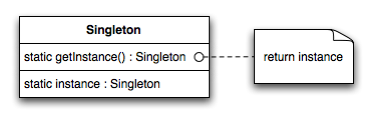
\includegraphics[scale = 0.6]{Singleton}
    \caption{Patrón \textit{Singleton} en Unity}
    \label{fig:Singleton} 
\end{figure} 

Con las referencias de los seis huesos creados, ahora lo que tocaría hacer es asignar el seguimiento de los sensores a cada hueso. Para ello es necesario crear un objeto de tipo \textit{VICIK} y un método denominado \textit{UpdateBoneReferences()} que realice la asignación para realizar la grabación de la captura de movimiento.

Con todo el escenario ya preparado para realizar la grabación del \textit{Mocap}, se creó la escena principal del proyecto, donde estarán todos estos componentes y scripts mencionados anteriormente. 

Para realizar la secuencia de grabación, se creo un panel en VR que permitiese grabar los movimientos a modo de estudio de grabación de música, con los tres botones clásicos (play, pause y stop), además de incluirse un panel para poder escribir el nombre del movimiento que se va a realizar.

El profesor podrá visualizar el movimiento que está realizado a cada instante, ya que verá una imagen de un avatar idéntico a él a modo de espejo, de este modo podrá revisar cada una de las poses que esté realizando mientras graba los movimientos que luego visualizará el alumno en la aplicación de AR. 

Cuando el profesor esté grabando un movimiento, podrá repetirlo las veces que consideré oportunas, finalizando la grabación con el botón de stop y volviendo a pulsar el botón de \textit{record} para iniciar de nuevo el proceso. También existe la opción de pausar una grabación, y retomarla instantes después antes de finalizar la grabación, pulsando el botón correspondiente (\textit{pause}). Cuando un movimiento se quiera reproducir antes de finalizar la grabación, existirá la opción de pulsar el botón de \textit{play}, siempre y cuando se haya pulsado el botón de \textit{stop} previamente. Tras toda esta secuencia, se habilitará un botón de finalizar para concluir la grabación del \textit{Mocap} y de nuevo se podría iniciar el proceso de grabación con un nuevo movimiento.

Los movimientos grabados serán guardados como animaciones de Unity, de modo que el profesor podrá visualizar los movimientos que haya grabado hasta el momento, para en el caso deseado, poderlo repetir y borrar el movimiento capturado previamente. Además, estos movimientos capturados serán los que se podrán analizar en el otro escenario del proyecto, el entorno del alumno en realidad aumentada.

\section{Análisis de \textit{Mocap} en AR}

Otra parte importante de este proyecto consiste en poder analizar los movimientos previamente grabados por el profesor, dependiendo del nivel del alumno. De esta manera se podrá realizar una corrección del movimiento que necesita practicar el alumno en tiempo real. En esta sección se explica cómo se ha desarrollado esta parte del proyecto con realidad aumentada.

\subsection{Investigación base}
\label{cap5:sec:panteamientoOpenCV} 

El planteamiento inicial sobre el análisis de los movimientos grabados por el profesor fue muy distinto al que finalmente se desarrolló. 

En la mayoría de las artes marciales los movimientos son repetidos miles de veces en cada sesión, es por esto clave optimizar el rendimiento para evitar lesiones y obtener unos resultados eficientes en su ejecución.

La evaluación de los movimientos de capoeira puede ser realizada por el ojo humano de un entrenador, con video análisis o con equipos de biomecánica especializados, como sensores de presión o programas tridimensionales que analicen los movimientos realizados. 

En primera instancia se estudió como realizar el análisis de los movimientos capturados por el profesor mediante \textit{Deep Learning} con\texttt{OpenCV}. Este sistema de visión artificial (descrito en la sección \ref{cap3:sec:OpenCV}) utiliza una serie de algoritmos basados en modelos (Ejemplos de modelos preentrenados en ImageNet: \textit{Xception, VGG19, ResNet50}) capaces de seguir la estructura ósea del movimiento del cuerpo humano. Este método se base en representar las partes del cuerpo humano en segmentos y unirlos mediante puntos, identificando principalmente el torso, la cabeza y las extremidades.

Visualizando la gran cantidad de estudios relacionados con \textit{OpenCV} y el análisis de movimientos, no dejaría de ser un estudio más sobre como analizar y aprender este tipo de arte marcial. Dado que la tecnología a evolucionado en gran medida en estos últimos años, se opto por utilizar una herramienta novedosa y en plena evolución, como es la realidad aumentada.

Para este apartado se observó el desarrollo realizado en VR sobre la grabación de movimiento explicada anteriormente. En esta sección el alumno podrá tener un\textit{feedback} visual inmediato y novedoso, de como poder realizar un movimiento de forma correcta en el arte marcial brasileño (capoeira).

Con el planteamiento de utilizar \texttt{AR} como base para el análisis de los movimientos del profesor y el posterior aprendizaje del alumno, se optó por desarrollar esta parte del proyecto con \texttt{ARCore} (ya se describieron los detalles de esta elección en la sección \ref{cap5:sec:ARCore}).

De todo el contenido incluido en el paquete de \texttt{ARCore} para Unity, se selecciona como ejemplo de estudio, \texttt{HelloAR}, dado el gran potencial que ha incluido \texttt{ARCore} en este escenario, un nuevo sistema de oclusión ambiental denominado \textit{Depth API}\footnote{\url{https://developers.google.com/ar/develop/unity/depth/overview}}. Este sistema utiliza la cámara RGB de los dispositivos móviles para crear mapas de profundidad, para posteriormente utilizar esta información y hacer que los objetos virtuales aparezcan con precisión 

Para entender un poco mejor como utiliza \texttt{ARCore} el sistema de profundidad vamos a explicar cómo realiza este proceso este \textit{SDK} de realidad aumentada (véase Figura \ref{fig:depth-values-diagram}). En la geometría del mundo real observamos un punto \texttt{A}, y un punto \texttt{a} 2D que representa el mismo punto pero en la imagen con el mapa de profundidad. El valor dado por esta \textit{API} es igual a la longitud de \texttt{CA} proyectada sobre el eje principal. Al trabajar con este sistema es importante destacar que los valores del mapa de profundidad no son la longitud del rayo \texttt{CA}, sino la proyección del mismo.

\begin{figure}[h!]
    \centering 
    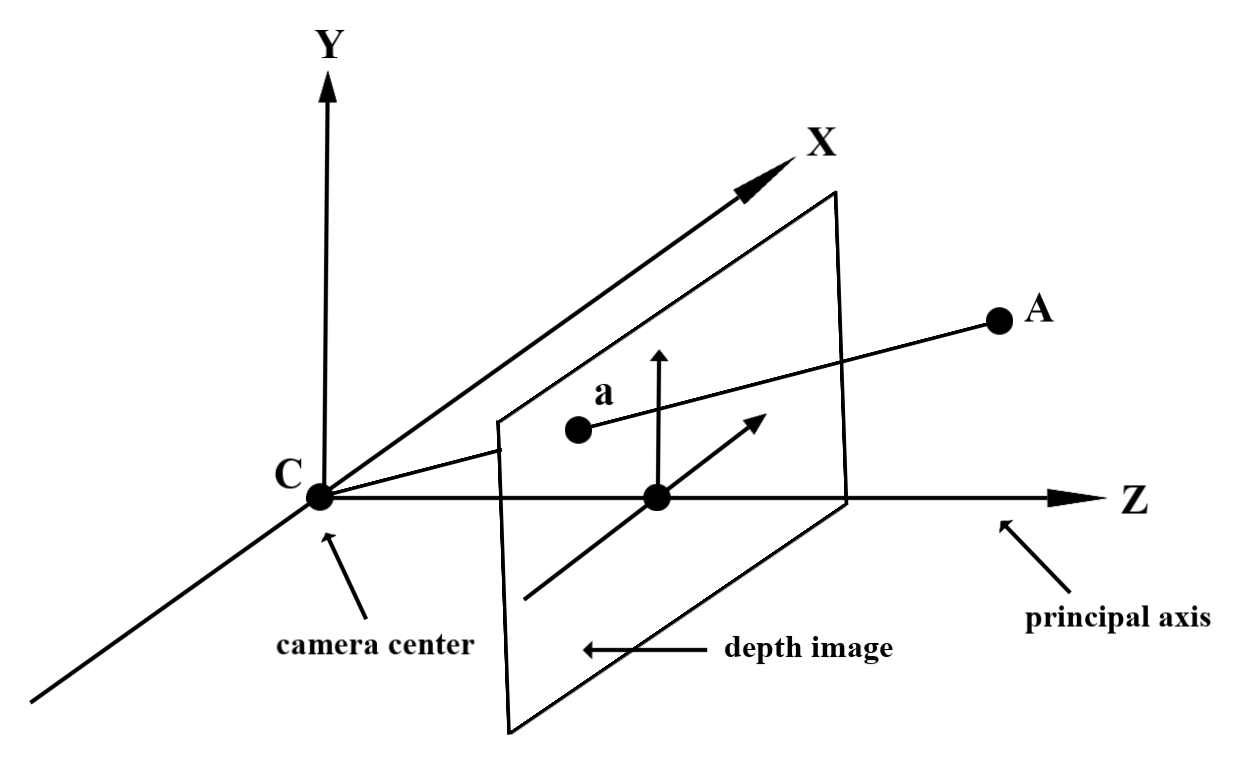
\includegraphics[scale = 0.2]{depth-values-diagram}
    \caption{Proyección en el plano utilizada en \textit{Depth API}}
    \label{fig:depth-values-diagram}
\end{figure} 

Ya en la escena de ejemplo \texttt{HelloAR} se visualiza como la API necesita tener un mapa del entorno a utilizar para poder colocar los objetos virtuales en el mundo real, permitiendo que \texttt{ARCore} establezca un seguimiento completo, detectando la geometría de la superficie con la que se quiere interactuar. Este proceso lo realiza el script \texttt{DetectedPlaneVisualizer} necesario en la utilización de este \textit{SDK}.

Otro de los scripts necesarios es \texttt{ARCoreSesion}, el cual determina cual de las dos cámaras (frontal o trasera) se utilizará en la aplicación a desarrollar. Además serán necesarios dos archivos de configuración denominados \textit{SesionConfig y CameraConfigFilter}. Estos archivos con extensión \textit{.asset de Unity} se utilizan para detallar la configuración de la cámara que \texttt{ARCore} utiliza para acceder al sensor de la cámara para una sesión determinada. Estos detalles incluyen, por ejemplo, la velocidad de fotogramas que captura el objetivo y si la cámara a utiliza un sensor de profundidad.

Al crear una nueva sesión de \texttt{ARCore}, este utiliza un filtro para determinar la configuración de la cámara que mejor coincida con la lista de configuraciones disponibles. Se puede utilizar el recurso \textit{CameraConfigFilter} para reducir las configuraciones de cámaras disponibles en una serie de dispositivos en tiempo de ejecución, según las necesidades de la aplicación.

Para esta escena de ejemplo, existe un script denominado \textit{HelloARController} el cual controla la instancia de la cámara a utilizar y como colocar los objetos 3D en el mundo real, pudiendo utilizar un plano vertical, uno horizontal o un punto fijo en el entorno. El problema radica en que este script instancia objetos 3D tantas veces como toques la pantalla, por lo tanto desarrollaremos un script propio denominado \texttt{ ARController} el cual se encargará de realizar una sola instancia del modelo 3D del profesor y otro script denominado \texttt{MovementManager} que gestionará de forma automática todos los movimientos grabados previamente en VR para ser asignados a la única instancia de la escena.

\subsection{Desarrollo del análisis de movimientos}

Después de haber realizado la investigación y compresión del material necesario para utilizar \texttt{ARCore} como sistema de realidad aumentada, se procede a solventar una serie de problemas o necesidades surgidas durante la investigación.

Para crear el entorno de AR, es necesario la utilización de uno de los \textit{prefabs} de \texttt{ARCore}, \texttt{ARCoreDevices} el cual incluye la configuración de la sesión a utilizar en realidad aumentada (\textit{SesionConfig y CameraConfigFilter}). En este escenario donde vamos a desarrollar una aplicación para el análisis visual de los movimientos grabados por el profesor en VR es necesario establecer unas configuraciones avanzadas detalladas a continuación:

\begin{itemize}
    \item \texttt{Config.PlaneFindingMode}: selecciona el comportamiento del sistema de superficie a detectar. En este desarrollo utilizaremos un sistema que solo detecte planos horizontales.
    \item \texttt{Config.CloudAnchorMode}: define una ubicación específica rastreada en el mundo real. De modo que guarda la posición real de objetos 3D para luego ser utilizados. En este desarrollo no utilizaremos esta opción, ya que no queremos tener un punto fijo para visualizar los movimientos del profesor.
    \item \texttt{Config.FocusMode}: tipo de enfoque de la cámara a utilizar, en los dispositivos compatibles como el utilizado para el desarrollo del proyecto, se utilizará el tipo \textit{Fixed} para optimizar el seguimiento en AR.
    \item \texttt{Config.DepthMode}: modo del mapa de profundidad a utilizar. En los dispositivos compatibles, la mejor profundidad posible se estima en función del hardware y software del dispositivo. Proporciona una estimación de profundidad para cada píxel de la imagen. El inconveniente es que agrega una carga computacional significativa. Para el desarrollo de este proyecto utilizaremos el modo \textit{Automatic} para que pueda ser utilizado en diferentes dispositivos.
\end{itemize}

Como ocurría en el escenario de VR, es necesario la utilización de un componente que actúa como un \texttt{Singleton} (véase la Figura\ref{fig:Singleton}), de modo que solo puede existir un objeto de tipo \texttt{FirstPersonCamera} en la escena. Este objeto como su propio nombre indica, se trata de la cámara que utiliza el sistema para mostrar toda la información desarrollada en realidad aumentada. Este componente estará incluido en el script que se describe a continuación.

Para realizar todo el control de la aplicación de AR, se desarrolló el script \texttt{ARController}. Este script controla los siguientes objetos de Unity necesarios para dar forma a esta aplicación:

\begin{itemize}
    \item \texttt{Objecto de tipo \textit{DepthMenu}}: tipo de Mapa de profundidad que se utilizará, se podrá activar o desactivar en todo momento en tiempo de ejecución (para que los dispositivos no compatibles con este sistema puedan utilizar la aplicación).
    \item \texttt{Objecto de tipo \textit{HorizontalPlanePrefab}}: se utilizará una instancia única cuando el alumno pulse la pantalla, siendo solamente utilizada para una superficie a detectar de tipo horizontal.
    \item \texttt{Objecto de tipo \textit{GameObject}}: este \texttt{Prefab} utilizará el método \texttt{Update()} de Unity (descrito en la sección \ref{cap4:sec:unity}) para detectar en cada \textit{frame} el instante preciso para crear el avatar del profesor, la posición, rotación y escala que tiene en cada momento dicho modelo 3D.
\end{itemize}

Para controlar toda la información obtenida en la grabación de movimientos en VR, se creó el script \texttt{MovementManager} capaz de gestionar la concurrencia existente entre los diferentes movimientos capturados por el \textit{Mocap}. En primer lugar, se creará una instancia única del avatar que utilizará el profesor del tipo \textit{Animator}, de este modo el siguiente paso a realizar será la asignación de forma automática de todos los movimientos grabados previamente. Esta asignación se realizará mediante una lista de tipo \textit{Animator} denominada \textit{movements} (List<Animator> movements). Para poder crear una asignación automática de los movimientos, es necesario crear un objeto \textit{AnimatorController} y un componente de Unity del mismo tipo. 

Teniendo todo esto, iniciamos el proceso de automatizar la asignación de los movimientos ya incluidos en la lista (ya que han sido importados en el proyecto, en una carpeta específica para tal fin). Para ello se creó un método denominado \texttt{AddMovementAnimator()} que recorre la lista y va asignado a modo de diagrama de estados, cada uno de los movimientos, con otro de ellos. De este modo, todos los movimientos podrán ser seleccionados una y otra vez en la interfaz de AR. 

\begin{figure}[h!]
    \centering 
    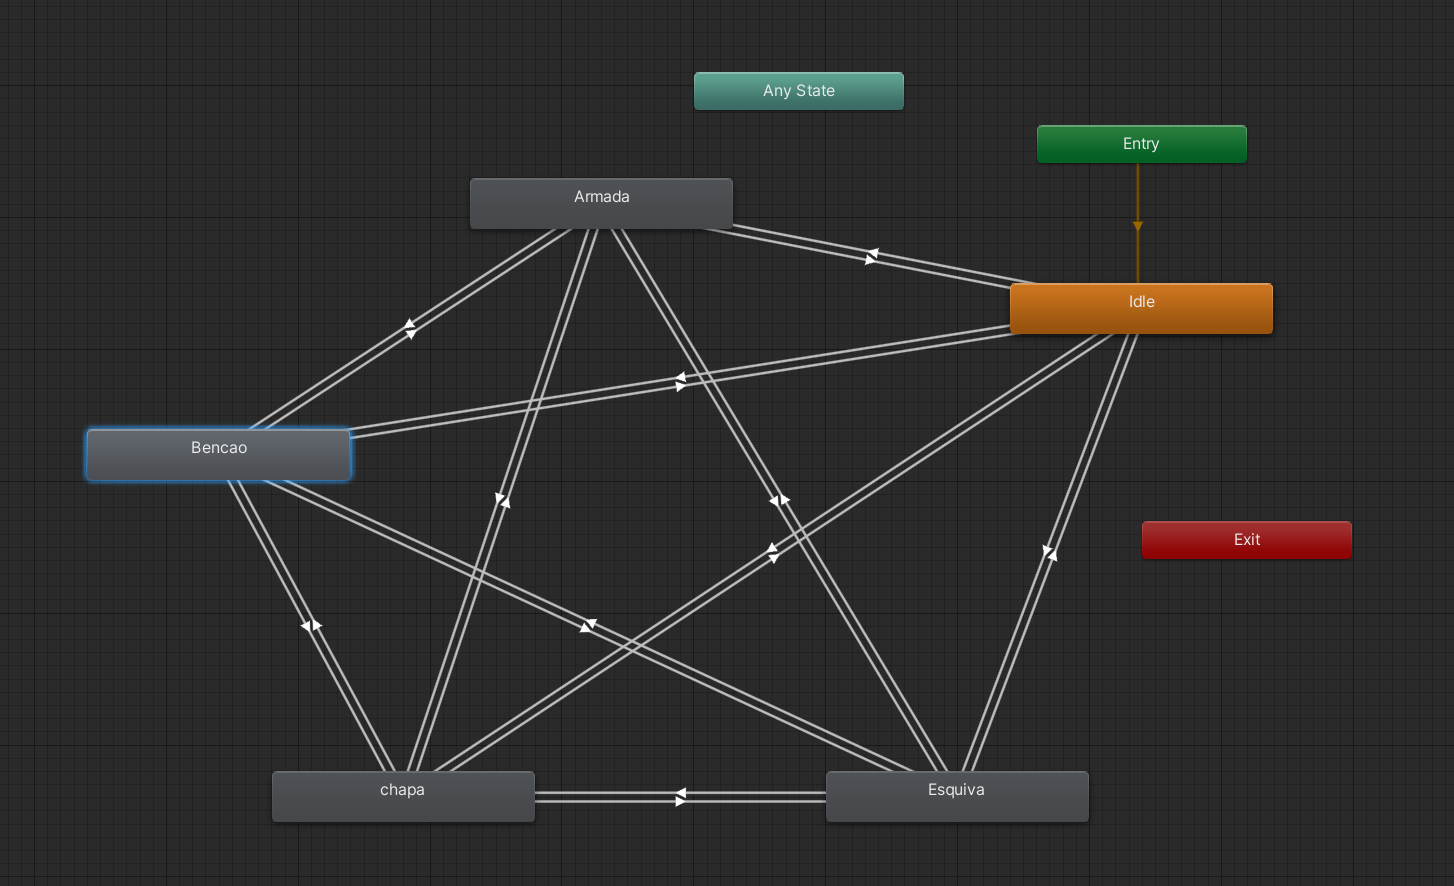
\includegraphics[scale = 0.5]{AnimatorController}
    \caption{Asignación automatizada de los movimientos grabados en el \textit{Mocap}}
    \label{fig:AnimatorController}
\end{figure} 

Además de todo este proceso, se creó un método el cual creará los botones de la interfaz en tiempo de ejecución denominado \texttt{MovementChanges()}, de este modo el método recorrerá la lista de movimientos guardados en la lista \textit{movements} y creará tantos botones en la \texttt{UI} como movimientos grabados existan, siempre dependiendo del nivel seleccionado previamente por el alumno.

En el planteamiento de como el alumno analizaría los movimientos grabados por el profesor para su posterior aprendizaje, se decidió que esta parte del proyecto se iba a desarrollar en realidad aumentada (como se explicó en la sección \ref{cap5:sec:panteamientoOpenCV}) debido a su gran potencial. 

Para este fin, se utilizó un sistema capaz de reproducir, pausar, aumentar y disminuir la velocidad del movimiento realizado por el profesor, para así poder analizar en 360º cada una de las poses que realiza el profesor para ejecutar la transición en cada movimiento del arte marcial brasileño (capoeira). El alumno podrá visualizar diferentes movimientos, dependiendo del nivel elegido al iniciar la aplicación, de modo que el profesor previamente ha grabado movimientos para todos los niveles seleccionables (principiante e intermedio). Todo este sistema ha sido desarrollado en un script denominado \textit{UIController}, creando instancias para cada uno de los botones seleccionables a la hora de reproducir los movimientos, además de los botones de reproducción, pause y el \textit{slider} capaz de aumentar el ritmo que utilizar el profesor en el movimiento capturado en VR.



Otro de los sistemas importantes a desarrollar para dar un efecto más realista es la utilización de la estimación de luz en AR, por defecto viene deshabilitada. Para este tipo de sistemas se pueden utilizar dos tipos de modos de luz ambiental, definidos a continuación:

\begin{itemize}
    \item \texttt{HDR Environmental}: el modo de estimación de luz se establece con o sin reflejos, de modo que el componente de luz ambiental en la escena actualizará la rotación y el color de la luz, además de modificar los componentes de Unity \textit{ambient probe} mediante la propiedad \texttt{RenderSettings.ambientProbe} y \textit{ reflection probe } mediante la propiedad \texttt{RenderSettings.customReflection}.
    \item \texttt{Ambient Intensity}: en este modo de estimación de luz, el componente de luz en la escena de Unity fijará \textit{\_GlobalLightEstimation} propiedad que se utiliza en la propiedad de\texttt{ARCore}  \texttt{DiffuseWithLightEstimation} y \texttt{SpecularWithLightEstimation} y otros \textit{shaders} personalizados para ajustar la salida de color final para que coincida con el color de la imagen de la cámara.
\end{itemize}

En el script denominado \texttt{ARController} se asigna mediante el método \texttt{SetLightEstimationMode()} el tipo de estimación de luz a utilizar en el proyecto de AR, pasandole al método de tipo \texttt{LightEstimationMode} el parámetro \texttt{EnvironmentalHDRwithReflections}.



\section{Diseño y creación de avatares}

En esta etapa del proyecto, con el objetivo de dar una sensación más realista al \textit{Mocap}, se han creado una serie de características estéticas en los avatares, siendo esta, similar a los profesionales que practican capoeira. De modo que la experiencia a proporcionar sea más amena para el usuario.

\subsection{Investigación base} 

En la búsqueda de software dedicado al modelado de personajes 3D se encontraron aplicaciones como \texttt{Blender}\footnote{\url{https://www.blender.org}}, \texttt{3ds Max}\footnote{\url{https://www.autodesk.es/products/3ds-max}}, \texttt{ZBrush}\footnote{\url{https://pixologic.com/}}, entre otras. 

Aunque la idea de esculpir en un escenario 3D puede sonar atractiva, ya que estos sistemas son capaces de crear objetos paramétricos y orgánicos con características de polígono, superficie de subdivisión y modelado basado en \textit{spline} (funciones utilizadas en aplicaciones de modelados 3D que requieren la interpolación de datos, o un suavizado de curvas). Las características interesantes (para los diseñadores en particular) son las herramientas de modelado basadas en NURBS (modelo matemático muy utilizado en programas de modelado 3D para generar y representar curvas y superficies), ya que en estos programas de diseño 3D permiten mallas orgánicas y matemáticamente precisas. Entre las otras técnicas está la capacidad de crear modelos a partir de datos de nube de puntos.

Este tipo de sistemas no son de ninguna manera programas de diseño 3D que puedas dominar intuitivamente. Tienen una curva de aprendizaje empinada, se necesitan muchas horas de práctica para dominar sus muchos pinceles y herramientas, sólo entonces es cuando se producen resultados satisfactorios. De modo que tienen una curva de aprendizaje demasiado larga para las necesidades dadas. 

También se examinó una aplicación llamada \texttt{MarvelousDesigner}\footnote{\url{https://www.marvelousdesigner.com/}} la cual se emplea para desarrollar prendas de vestir. El problema surgía cuando se intentaba importar el avatar creado con \texttt{Fuse Character Creator }, ya que no eran compatibles los formatos de las dos aplicaciones y por lo tanto se descartó seguir por esta vía. 

En el camino se observó que existía una aplicación para el desarrollo de avatares compatibles con una solución de captura de movimiento y a su vez, un entorno dedicado a la conexión entre la creación de modelos 3D y el ajuste de rigueado que debe tener un avatar para este proyecto. Por este motivo, se tomó la decisión de utilizar \texttt{Adobe Fuse Character Creator}\footnote{\url{https://www.adobe.com/es/products/fuse.html}} como aplicación para el desarrollo de los personajes, ya que se amoldaba perfectamente a las necesidades de este proyecto.

\subsection{Diseño de los avatares}

Con el objetivo de crear un entorno más realista, se crearon dos avatares diferentes, cada uno con una estética propia. A la hora de elaborar el vestuario de los personajes, se observó la vestimenta utilizada por los integrantes de escuelas que practican este arte marcial brasileño. Se trata de un pantalón largo y una camiseta o sudadera en color blanco. 

Con el propósito de crear una ropa muy similar a la utilizada en capoeira, se usaron prendas prediseñadas en la aplicación \texttt{Adobe Fuse Character Creator} como los pantalones, camisetas y sudaderas que utilizarían los avatares del sistema con los retoques apropiados para darle ese color blanco característico de este arte marcial.

\begin{figure}[h!]
    \centering 
    \includegraphics[scale = 0.6]{Rigger}
    \caption{Auto-Rig con 65 huesos de Mixamo}
    \label{fig:Rigger}
\end{figure} 

Tras completar la estética de los personajes, \texttt{Adobe Fuse Character Creator} ofrece la posibilidad de configurar los huesos de los avatares para posteriormente iniciar el proceso de rigueado que suministra \texttt{Mixamo}. La misma aplicación \texttt{Adobe Fuse Character Creator} proporciona el servicio de conexión con \texttt{Mixamo}, de modo que solo sería necesario seleccionar la opción de la aplicación para subir los avatares creados a los servidores de \texttt{Mixamo}. Cuando se complete este proceso, la aplicación redirigirá su actividad al navegador web. 

\texttt{Mixamo} también ofrece la posibilidad de crear varios esqueletos para un mismo avatar, en este caso se presentan cuatro posibles escenarios dependiendo de las necesidades dadas con 25, 41, 49 y 65 huesos respectivamente (véase Figura \ref{fig:Rigger}). La diferencia mayoritariamente depende de los huesos que queremos que tenga el avatar en las manos.

Una vez investigada la generación y construcción de los huesos de los avatares. El avatar elegido que mejor se adapta a este \texttt{Mocap} es el que contiene 65 huesos, ya que demuestra una movilidad correcta y en el futuro podrá ser usado en sistemas de captura de movimiento incluyendo \textit{hand tracking} (véase Figura \ref{fig:HandTracking}) (sistema por el cual, una serie de cámara colocadas en las gafas de VR o AR detectan cualquier movimiento realizado con las manos).

\begin{figure}[h!]
    \centering
    \animategraphics[loop,autoplay,width=0.8\linewidth]{10}{/HandTracking/HandTracking-}{0}{80}
    \caption{\textit{Hand tracking} en Oculus Quest}
    \label{fig:HandTracking}  
\end{figure}





